\chapter{Exploiting Parallelism}

\section{Static Scheduling}
Dynamic scheduling (out of order scheduling) requires significant hardware complexity.
\begin{itemize}
	\item Register Update Units, reorder buffers, registers backed by commit registers and associated with tags, instruction dependency checks.
	\item All of these take space on the die (not only does a larger chip necessitate fewer chips per wafer, but the yield is also decreased)
	\item Also requires more energy, results in more heat and hence lower thermal limits.
	\item The complexity of determining the number of instructions that can safely be issued in parallel is $O(n^2)$, which is achievable for small $n$, but can necessitate more stages between fetch and issue.
\end{itemize}
With static scheduling this complexity is removed from hardware, and moved to the compiler, with the ISA providing necessary mechanisms to express how instructions should be scheduled (e.g in parallel).

\subsection{Software Pipelining}
\begin{center}
	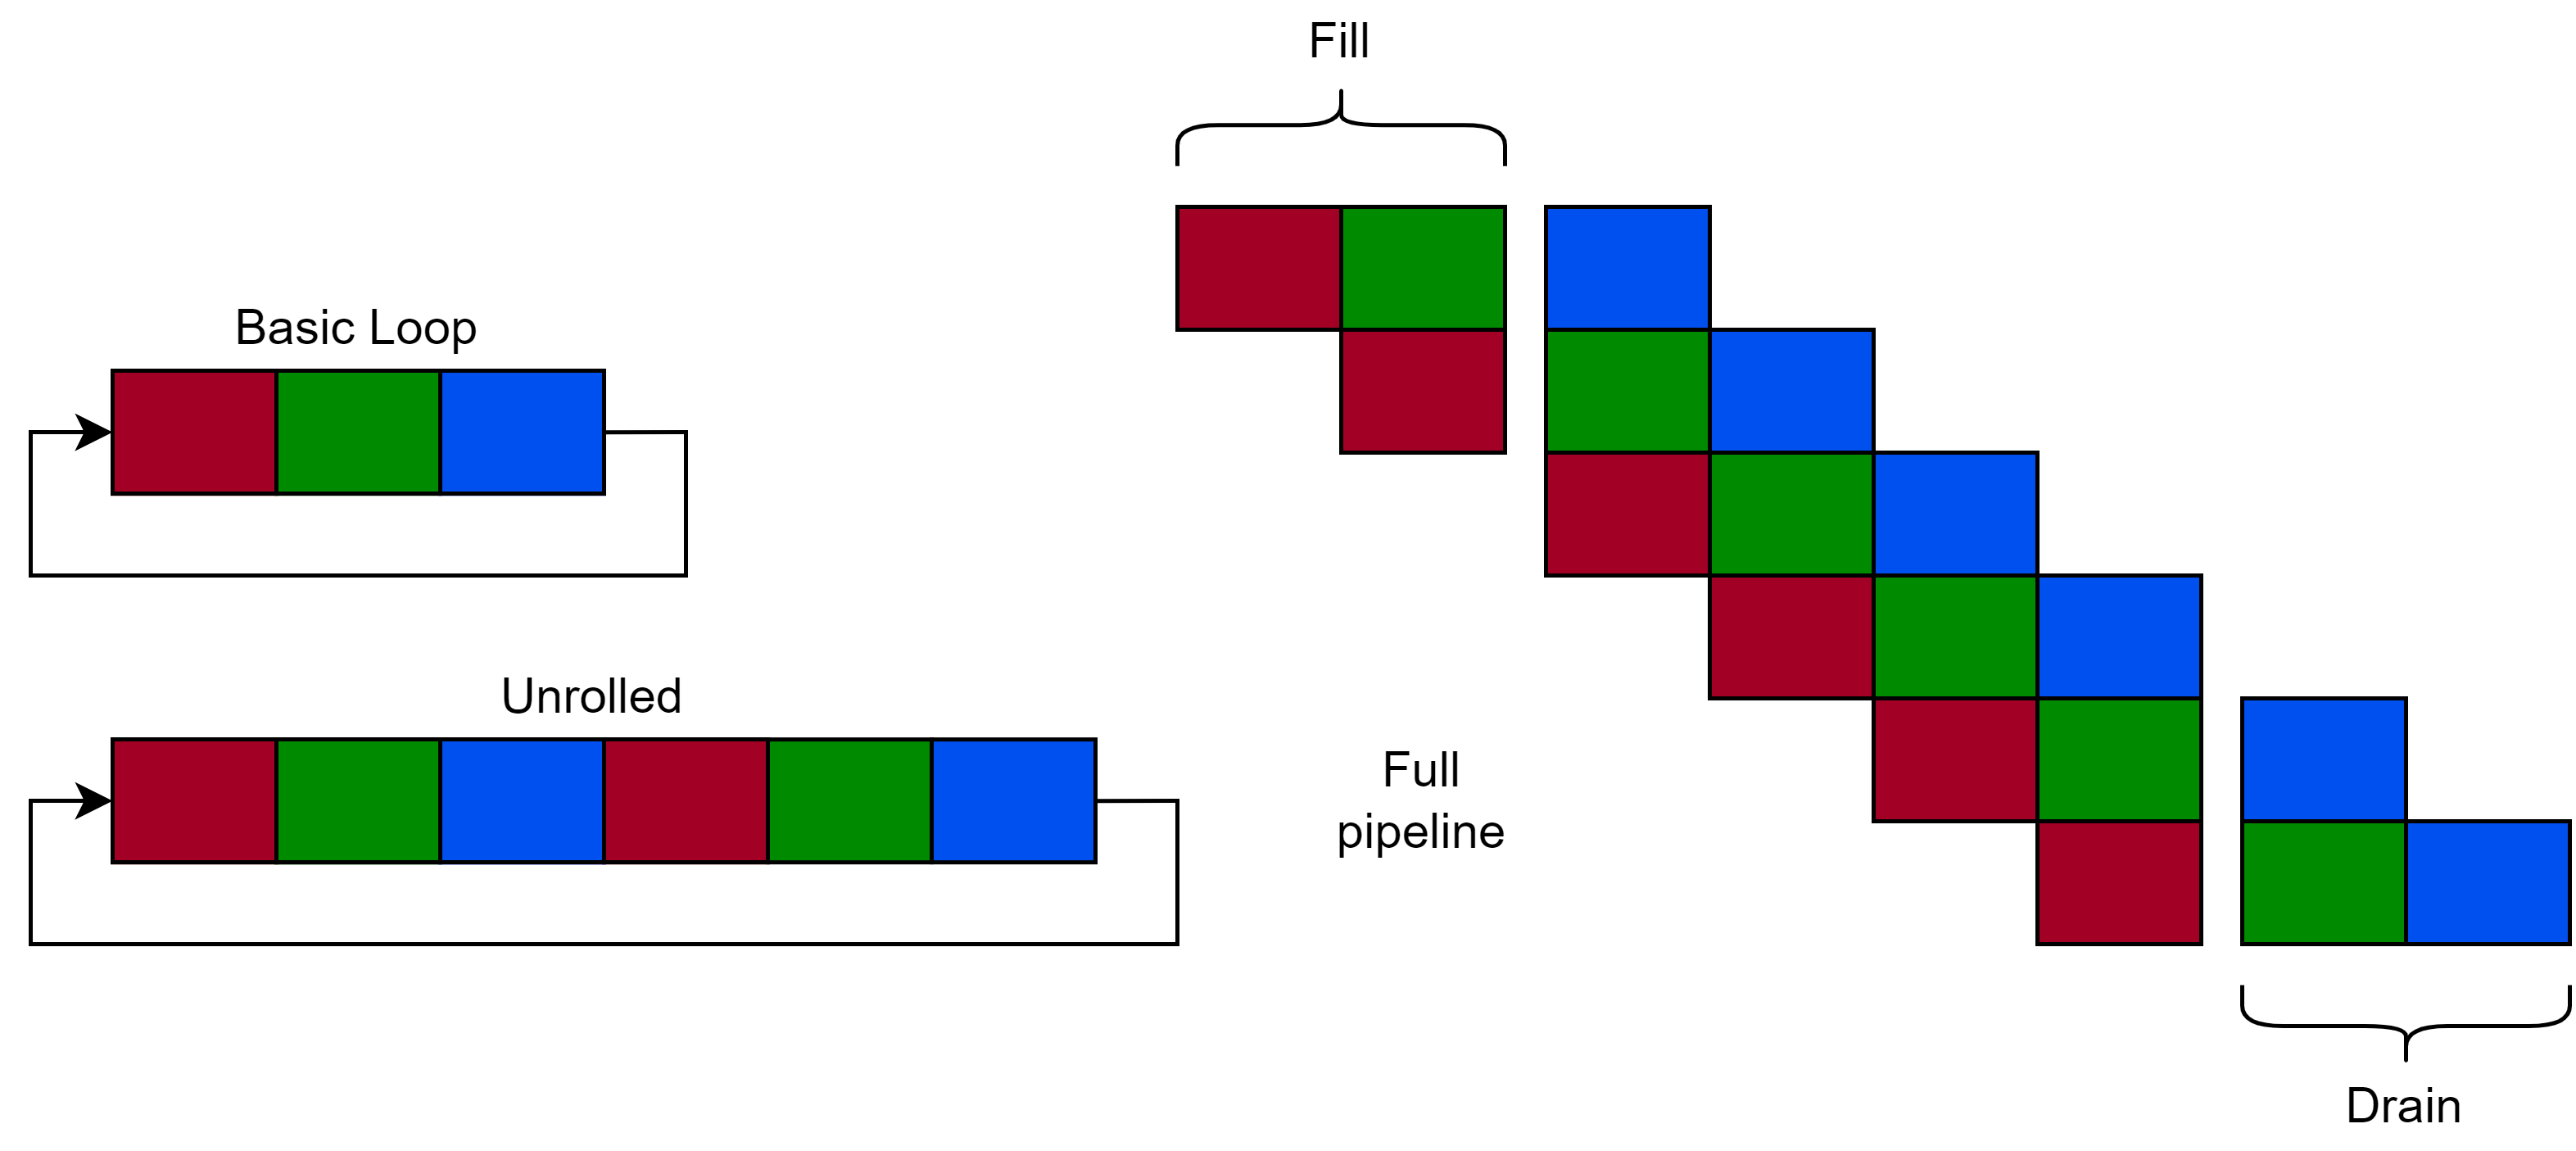
\includegraphics[width=\textwidth]{exploiting_parallelism/images/software_pipelining.drawio.png}
\end{center}

We can pipeline loop iterations, in the diagram above the basic loop and unrolled loop both execute the loop contents in order. By pipelining each of the 3 instructions in the loop body are run for 3 different in-order \textit{iterations}.
\begin{itemize}
	\item e.g iteration $3$ is in red, while $2$ is in green and $1$ is in blue.
	\item Increases the load-use distance, so removes/reduces stall potential.
\end{itemize}

\subsection{Very Lond Instruction Word}
\begin{definitionbox}{Very Lond Instruction Word (VLIW)}
	Each instruction contains encodings for multiple operations.
	\begin{itemize}
		\item All operations are independent and hence can be issued and executed in parallel.
		\item The compiler/programmer needs to extract dependencies, and work out which instructions can be issued \& executed in parallel, rather than the hardware.
		\item Instructions become large, and where there is little parallelism to be extracted, majority of the instructions are mostly no-ops.
		\item Large instructions put pressure on memory access bandwidth.
		\item Often not binary compatible across generations (e.g number of functional units change, instruction size changes)
	\end{itemize}
\end{definitionbox}
With software pipelining we can schedule instructions for different stages of the pipeline in parallel.

\subsection{Explicitly Parallel Instruction Computing}
\begin{definitionbox}{Explicitly Parallel Instruction Computing (EPIC)}
	A term created by Intel \& HP, considered to be the next generation of VLIW.
	\begin{itemize}
		\item Often used to refer to IA-64 (Itanium) processors.
		\item ISA exposes parallelism to the compiler.
		\item Binary compatible across generations/processor implementations.
	\end{itemize}
\end{definitionbox}

In IA-64 instructions are encoded in bundles, each 128 bits wide:
\begin{itemize}
	\item $5$ bit template field encodes which instructions can be run in parallel in the bundle (where the $;;$ / $stop!$ is, after which the next set of parallel instructions begin)
	\item $3$ instructions, each with $41$ bits of length, this allows for large number of registers, large immediate operands.
\end{itemize}
\subsubsection{Rotating Register File}
\begin{itemize}
	\item Registers $0$ to $31$ are always accessible.
	\item Registers $32$ to $128$ can rotate.
\end{itemize}
This allows for two main advantages:
\begin{center}
	\begin{tabular}{p{.2\textwidth} p{.8\textwidth}}
		\textbf{Register Stack}                        & By using a special register CFM (current frame pointer) to point to the set of registers used by a procedure. This allows many register arguments to be used for function calls, with results placed in registers in a stack like fashion. \\
		\textbf{Improved \newline Software Pipelining} & As the registers can be \textit{rotated} we can pipeline loops more easily (register names remain the same, but values rotated for each loop iteration).                                                                                   \\
	\end{tabular}
\end{center}
\begin{minted}{asm}
# Branch to L1, and rotate the register file by 1.
br.ctop <label> ;;
\end{minted}

\subsubsection{Predication}
There are $64$, single bit registers that can be used to determine whether an instruction is run.
\begin{itemize}
	\item Branches can be eliminated in favour of predicated instructions (can hence avoid branch \& branch mispredict costs)
	\item Can issue both sides of a branch in parallel \& predicate both.
	\item Can easily move instructions across conditional branches.
\end{itemize}

\subsubsection{Speculative Loads}
\begin{itemize}
	\item Compiler can specify speculative loads, and specify when loads will be used.
	\item Reduces cycles wasted to load-use stalls.
	\item Speculative loads do not fault, and hence can safely be used in code containing branches (e.g check if a pointer is null, can speculatively load before null check, but never use the value)
	\item An \textit{advanced load} variant checks for aliasing stores (stores to same location)
	\item An \textit{advanced load address table} tracks stores to addresses of \textit{advanced loads}
\end{itemize}
\begin{minted}{asm}
# Speculatively load r1 = *a
ld.s r1=[a]

# If the load for r1 faulted, go to some other branch, else NOP
chk.s r1 

# r1 value made non-speculative and can now be used.
use=r1

# An advanced speculative load, monitors the address b for loads
ld.a r2=[b]

# A store occurs to address b
st ??? [b]

# If aliasing has occurred for b, then re-load it
ld.c r2=[b]

use=r2
\end{minted}

When speculative loads are not fulfilled (i.e due to a fault - e.g page fault) \textit{NaT} (Not a thing) is placed in the destination register.
\begin{itemize}
	\item Speculatively loaded data can be consumed by other instructions before use.
	\item The \textit{NaT} is propagated until checked.
\end{itemize}

\unfinished

\section{Multithreading}

\lectlink{https://imperial.cloud.panopto.eu/Panopto/Pages/Viewer.aspx?id=b718ce56-8ebd-4d51-b886-af2a0112a4c5}{Chapter 7: Multithreading}

\begin{center}
	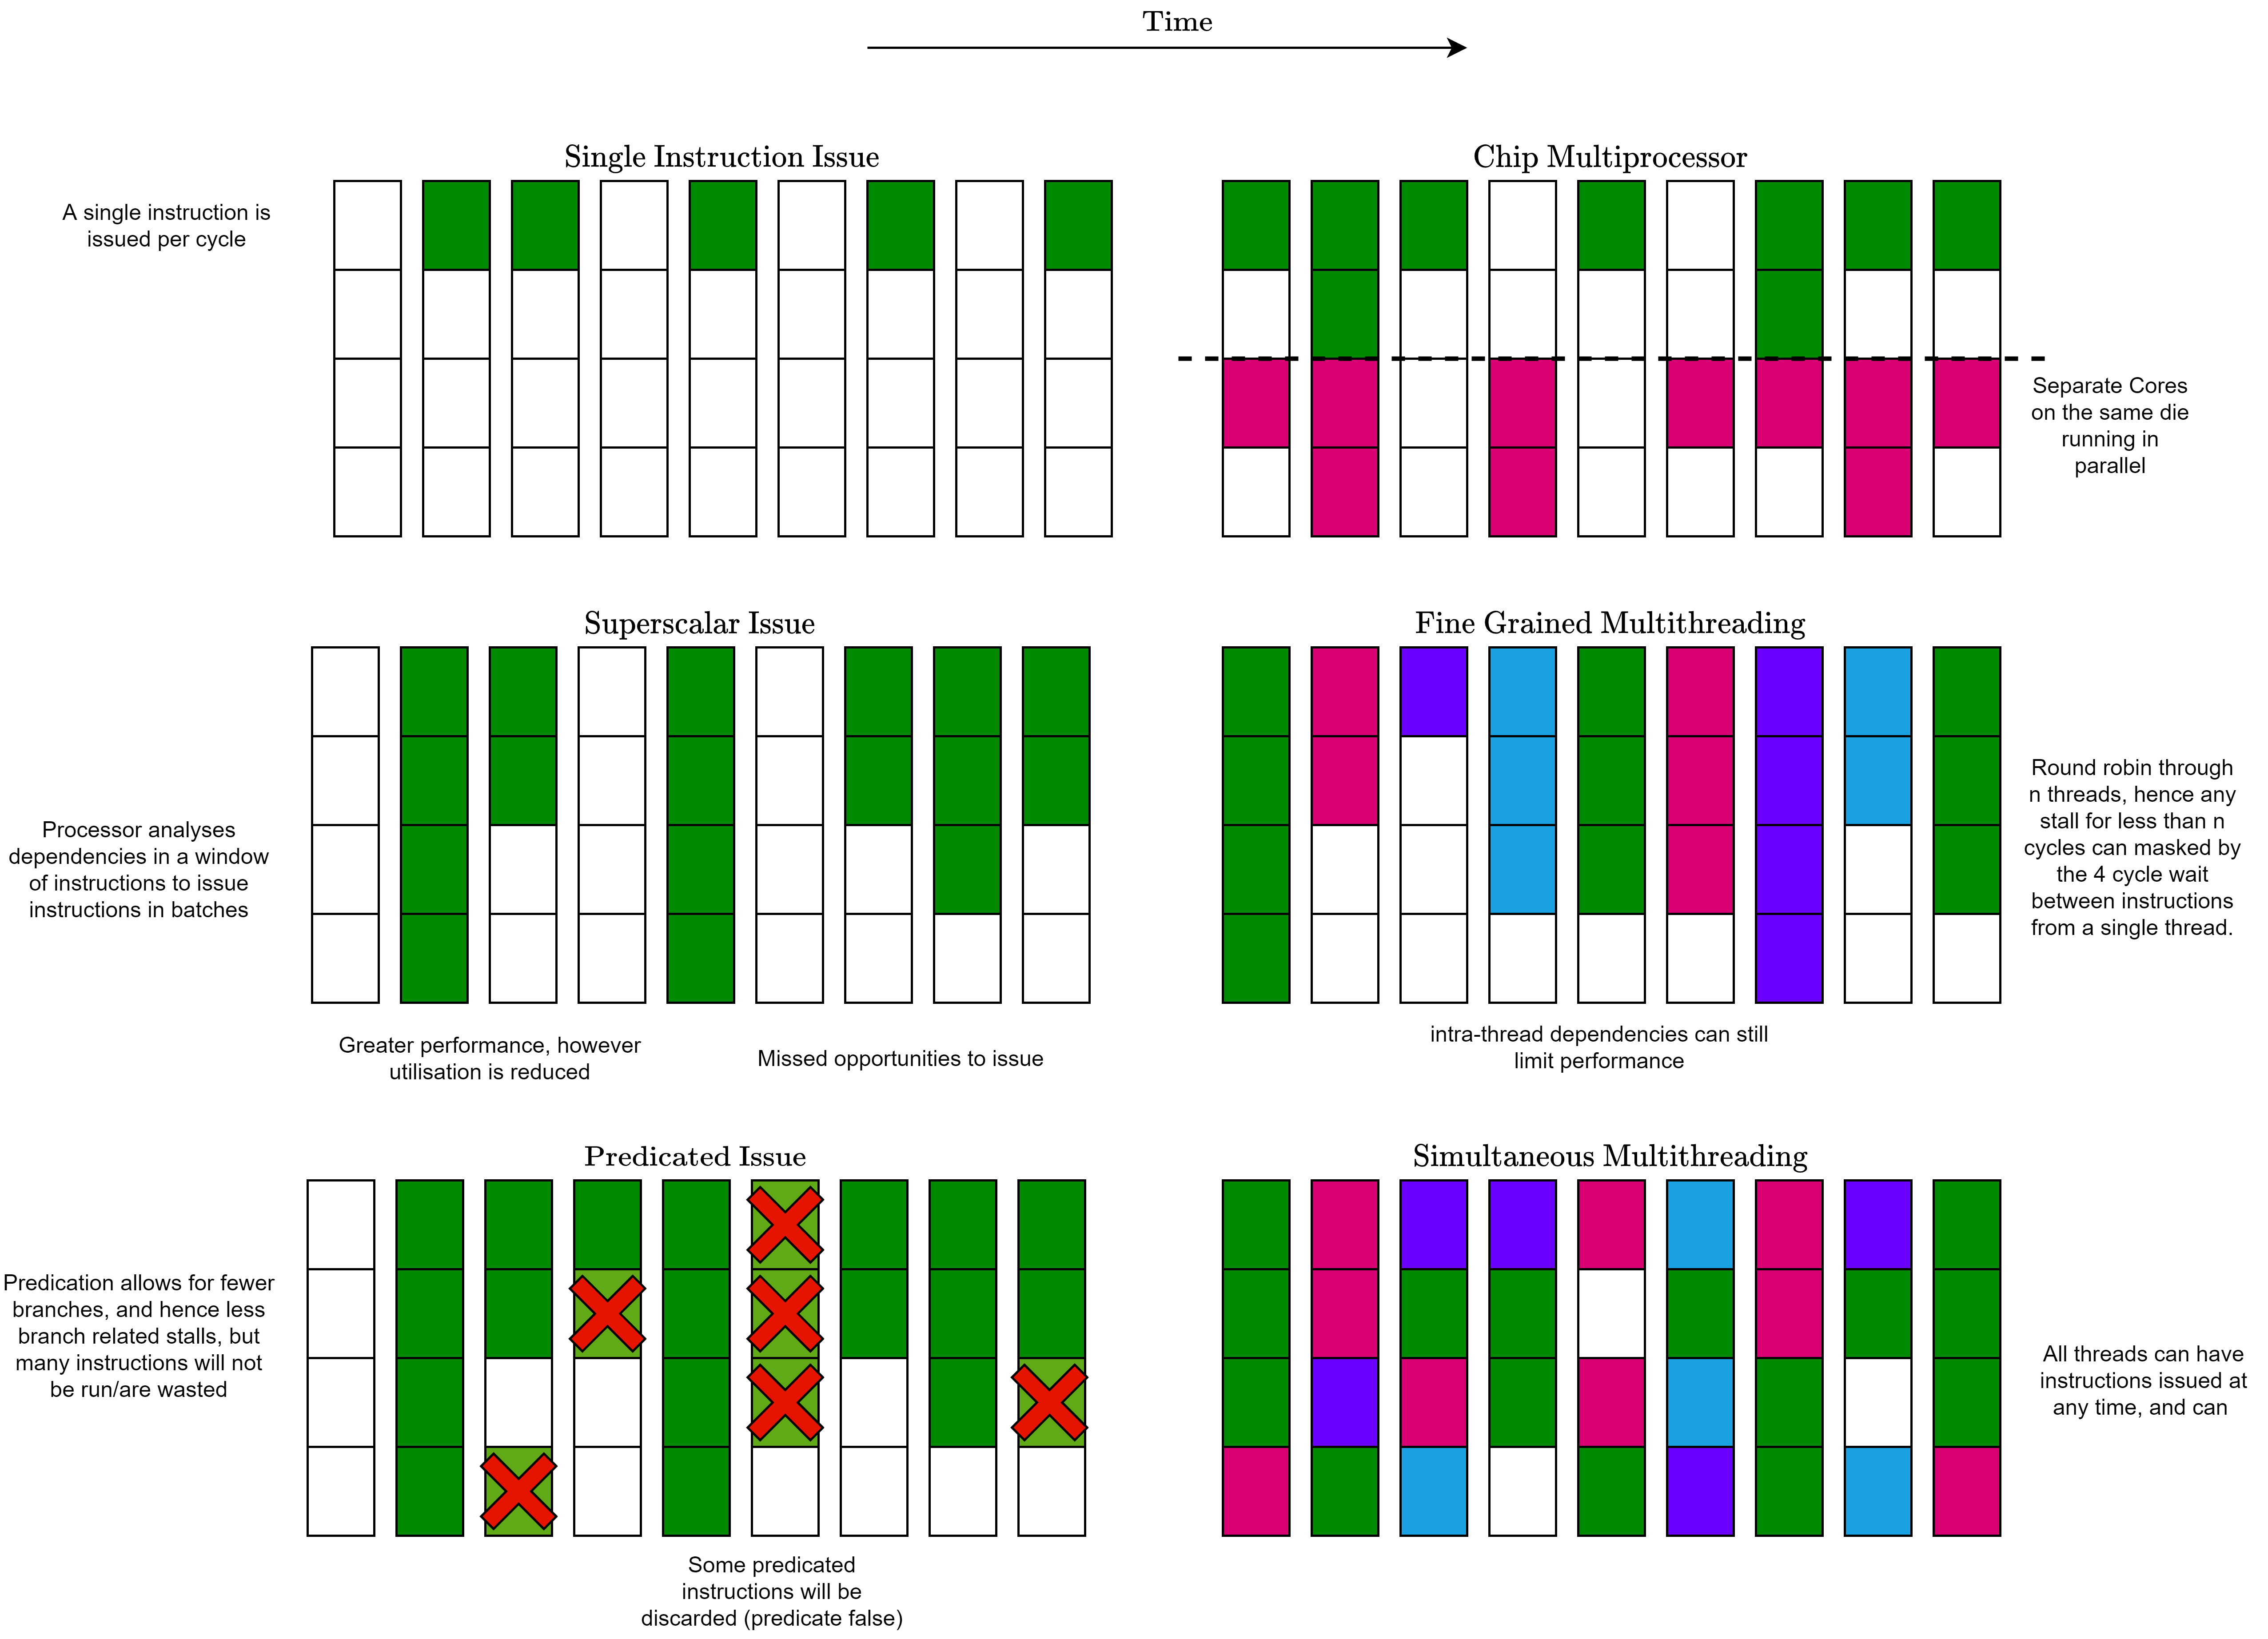
\includegraphics[width=\textwidth]{exploiting_parallelism/images/issues.drawio.png}
\end{center}
\begin{definitionbox}{Fine Grained Multithreading (FGMT)}
	Each cycle one thread can issue instructions.
	\begin{itemize}
		\item Typically round-robin through threads.
		\item Hence can \textit{hide} a stall of $n$ cycles for $n$ threads.
	\end{itemize}
\end{definitionbox}

\subsection{Simultaneous Multithreading}
\begin{definitionbox}{Simultaneous Multithreading (SMT)}
	Where instructions from several threads can be issued in any cycle.
	\begin{itemize}
		\item Requires a more complex frontend (e.g to tag cache entries with which thread they are for, TLB needs to know page table per thread)
		\item Instructions can be scheduled from any of the threads, maximizing utilisation.
		\item Threads may contest resources (i.e two threads want to use the same functional units) resulting in reduced performance for a thread, conflicts in the cache.
		\item Side channel attacks are an issue (threads share cache, scheduler needs to prevent one thread monopolising the CPU)
		\item Some resources do not need to be replicated for each thread (e.g can have $n$ times more logical registers, but not actual registers, one thread can use more than $\sfrac{1}{n}$ of the cache)
	\end{itemize}
\end{definitionbox}

SMT can allow for memory-system parallelism to be exploited
\begin{itemize}
	\item Lots of threads can have memory accesses \textit{in-flight}.
	\item Can overlap data accesses with computation from other threads (e.g issue from thread $B$ while $A$ is stalled on a load-use)
\end{itemize}

\unfinished

\section{Vector Processing}

\lectlink{https://imperial.cloud.panopto.eu/Panopto/Pages/Viewer.aspx?id=501d4469-4bb5-4076-9f0d-af2a0112d1b4}{Chapter 8: Vector Instructions and SIMD}

\subsection{Arithmetic Intensity}
\begin{center}
	
\includegraphics[width=\textwidth]{exploiting_parallelism/images/arithmetic_intensity.drawio.png}
\end{center}
\begin{itemize}
	\item Arithmetic intensity compares the ratio of arithmetic operations to memory operations.
	\item Hence we can determine if a program is limited by the rate of arithmetic operations, or by the memory bandwidth.
	\item FLoating point arithmetic is often used in this context, where arithmetic intensity is a measure of $FLOPs/Byte$
\end{itemize}
\begin{center}
	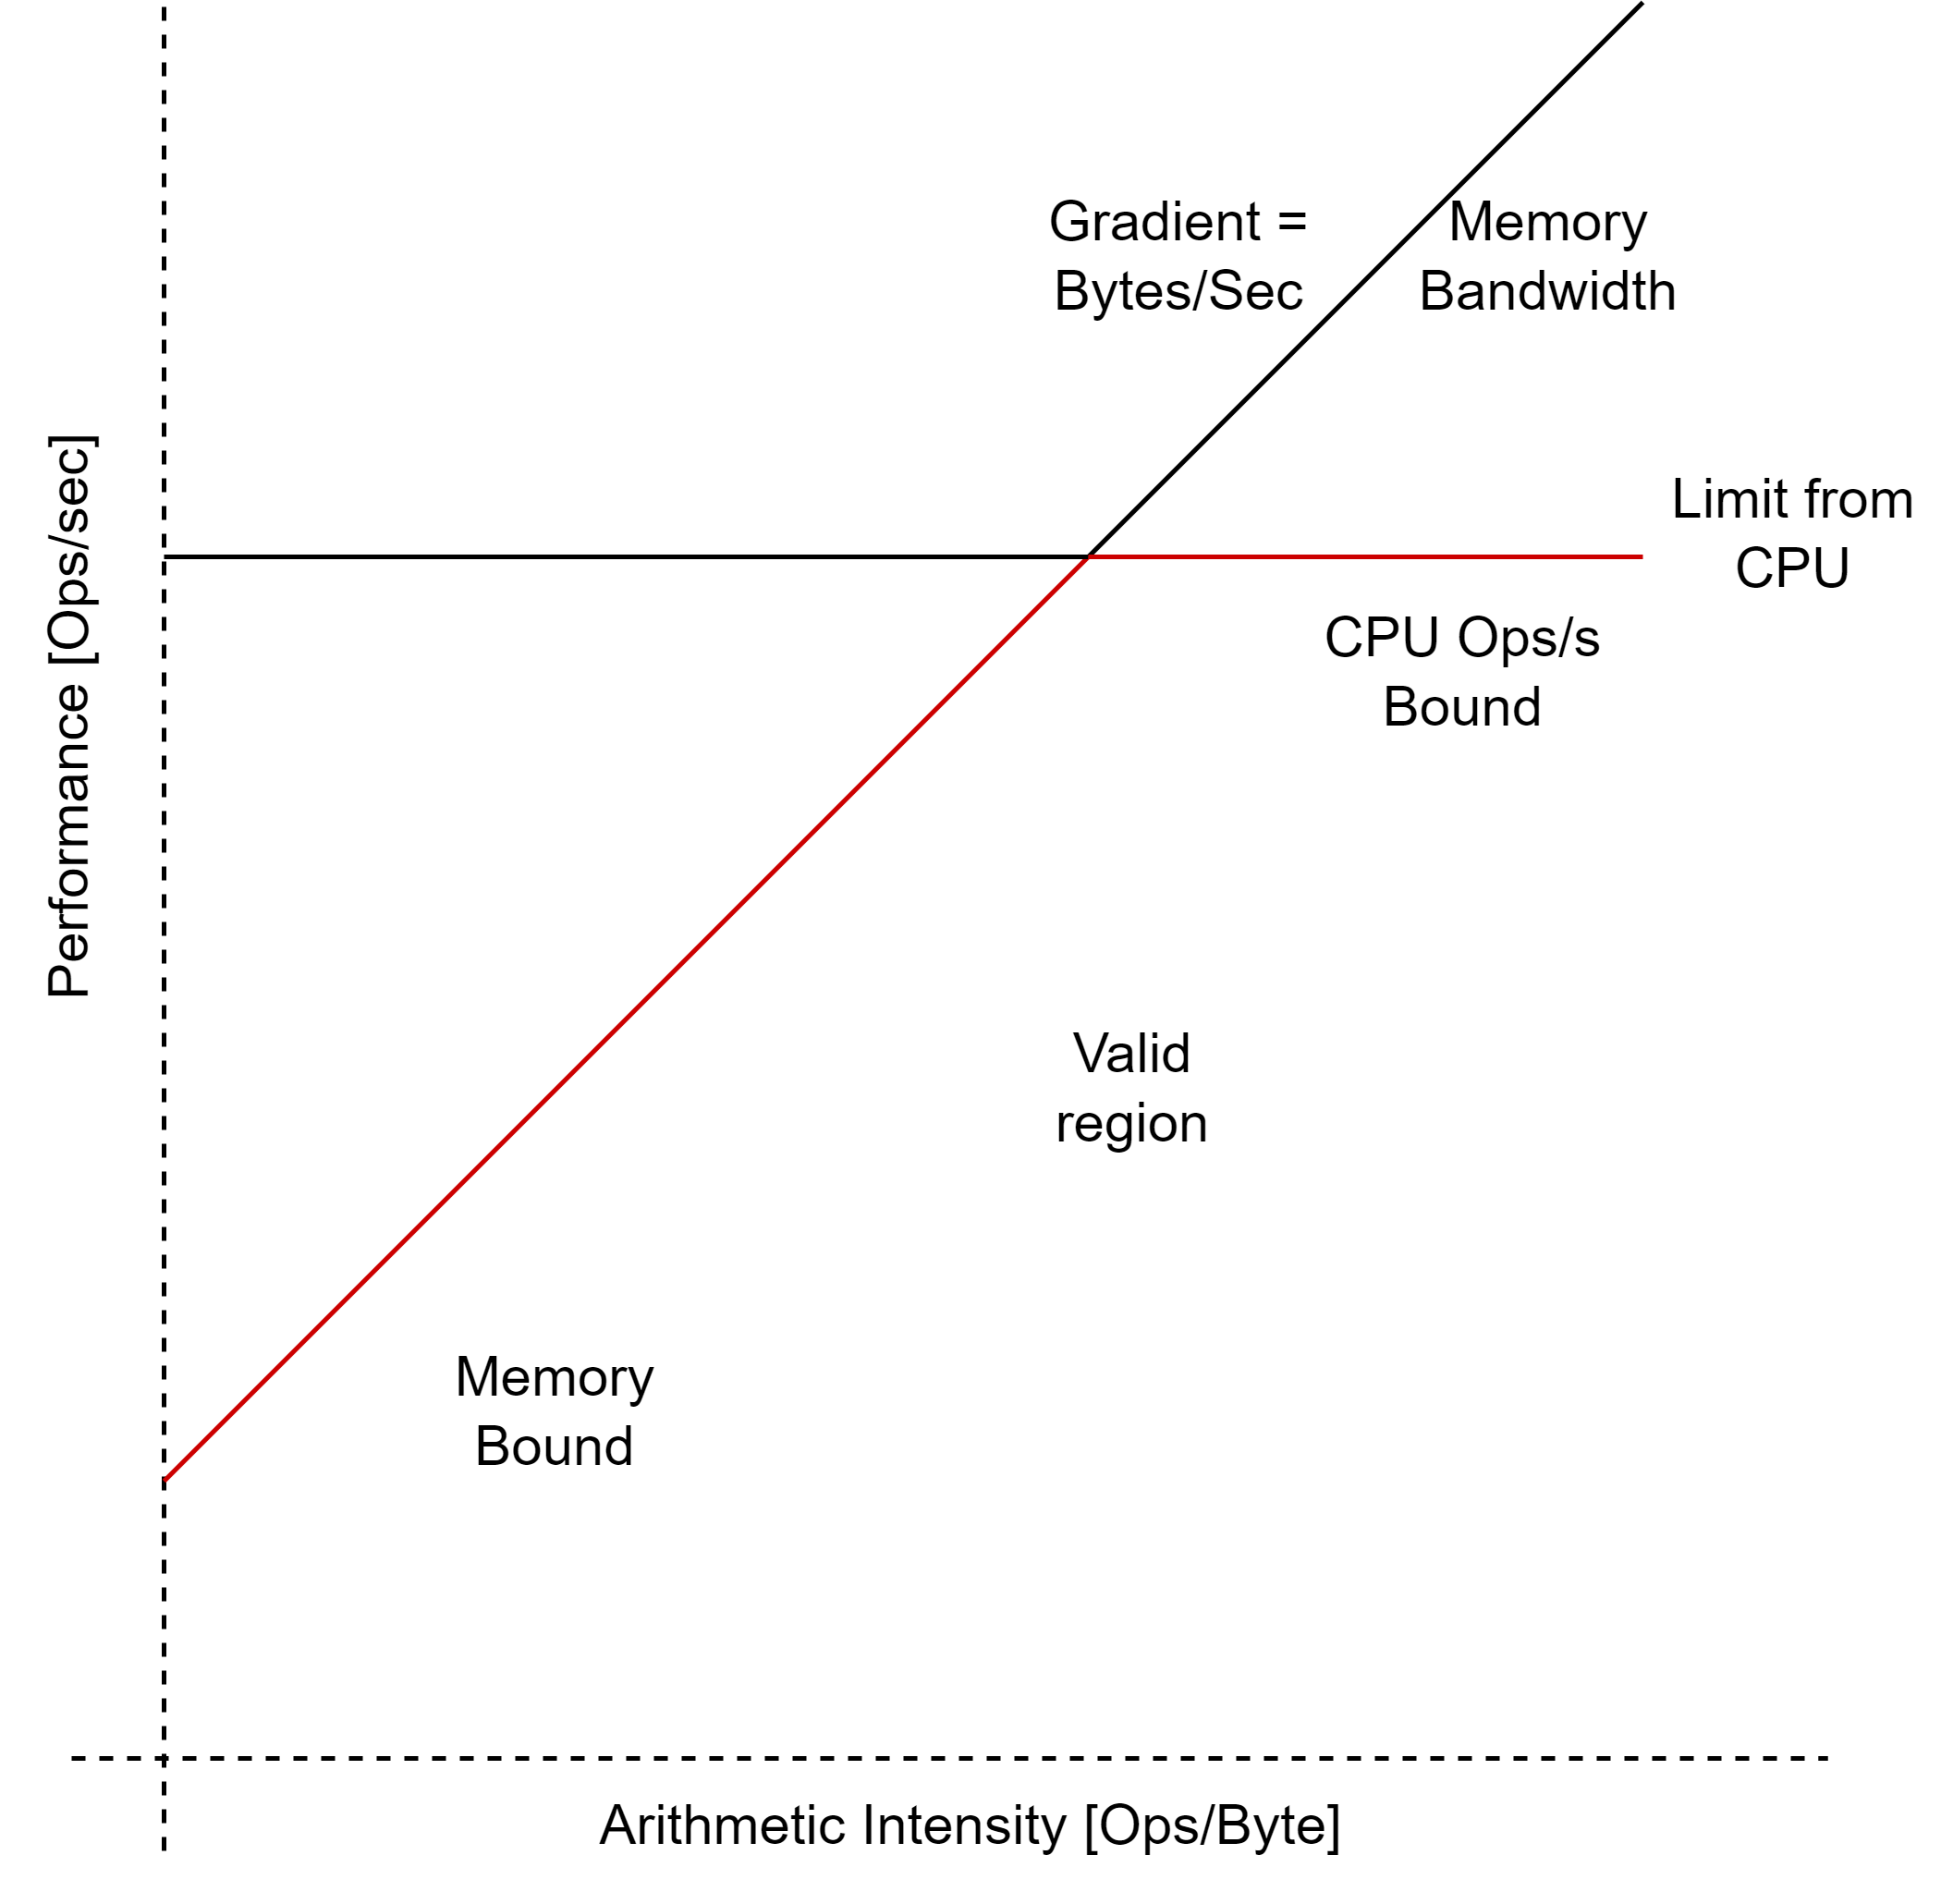
\includegraphics[width=.6\textwidth]{exploiting_parallelism/images/roofline_model.drawio.png}
\end{center}

\subsection{Vector Instruction Set Extensions}
\begin{definitionbox}{Intel AVX-512}
	A vector extension for Intel's x86-64 architecture.
	\begin{itemize}
		\item 32 extended registers (ZMM0 $\to$ ZMM31), each is $512$ bits wide.
		\item Can use registers to store 8 doubles, 16 floats, 32 shorts or 64 bytes.
		\item Instructions are executed in parallel in $4,32,16$ or $8$ \textit{lanes}.
		\item Predicate registers (k0 $\to$ k7 where k0 is always true), each predicate register holds up to $64$ bits and hence each register can hold a predicate per \textit{lane}
	\end{itemize}
\end{definitionbox}

\begin{definitionbox}{Compiler Intrinsics / Built In Functions}
	Subroutines available for use in a given language, with an implementation handled by the compiler.
	\begin{itemize}
		\item Often related to performance - e.g software prefetching.
		\item Used where the language cannot express some constraints / semantics - e.g vector instructions \& C
	\end{itemize}
\end{definitionbox}

Compiler intrinsics are provided for emitting specific vector instructions. For example with AVX12:
\begin{minted}{C}
#include <immintrin.h>

// we can now use compiler instrinsic
res = _mm512_maskz_add_ps(k, a, b)
\end{minted}
\begin{minted}{asm}
# Instead of assembly
VADDPS zmm1 {k1}{z}, xmm2, zmm3
\end{minted}
Conditionals may be required in vectorised code, to allow this the predicate registers are used to determine the results of their corresponding lanes.
\begin{center}
	\begin{tabular}{l l p{.8\textwidth}}
		\textbf{Zero Masking} & \mintinline{C}{z or {z}} prefix & Inactive lanes produce a zero                    \\
		\textbf{masking}      & No prefix                       & Inactive lanes do not overwrite previous result. \\
	\end{tabular}
\end{center}

The compiler must consider several issues in order to vectorise even simple code:
\begin{minted}{C}
void add(int *a, int *b, int *c) {
    for (int i=0; i < N; i++)
        c[i] = a[i] + b[i]
}
\end{minted}
\begin{center}
	\begin{tabular}{l p{.8\textwidth}}
		\textbf{Aliasing}  & In the above example a and b may overlap with c. We can inform the compiler these are separate using \mintinline{C}{restrict}. Otherwise the compiler may need to generate code that checks for aliasing, and only runs vectorised code if the arrays are distinct. \\
		\textbf{Size}      & The size may not be a size supported by vectorisation (here we can have $16$ elements), may vector instructions may be needed (in a loop), and for a non-power-of-two extra loop code may be required.                                                              \\
		\textbf{Alignment} & The vectorised load typically requires some alignment (e.g on a 32 byte boundary), extra code may need to check this alignment and sequentially execute part of the start/end of the loop.                                                                          \\
	\end{tabular}
\end{center}
Ultimately the compiler may not be able to vectorise a loop. We can use tools like OpenMP to tell/ask the compiler to vectorise code, even if it cannot assure this is safe.
\begin{minted}{C}
// To inform the compiler vectorisation is safe (it may not vectorise)
void add(float *a, float *b, float *c) {
    // Ignore Vector DEPendencies / assume no loop-carried dependencies
    #pragma ivdep
        for (int i = 0; i <= N; i++)
            c[i] = a[i] + b[i]
}

// To tell the compiler to vectorise the code (it may still not - e.g call 
// non-vectorisable function from within loop told to bve vectorised)
void add(float *a, float *b, float *c) {
    // OpenMD make this loop SIMD
    #pragma omp simd
        for (int i = 0; i <= N; i++)
            c[i] = a[i] + b[i]
}

// We can also make functions vectorisable, hence this function can be called 
// from a vectorised loop
#pragma omp declare simd
void add_element(float *a, float *b, float *c) {
    *c = *a + *b
}
\end{minted}
If the compiler still will not vectorise, we can rely on intrinsics:
\begin{minted}{C}
void add(float *a, float *b, float *c) {
__m128* pSrc1 = (_m128*) a;
__m128* pSrc2 = (_m128*) b;
__m128* pDst = (_m128*) c;

// lengths are part of data types
for (int i = 0; i <= N / 4; i++, pSrc1++, pSrc2++, pDest++)
    *pDest = _mm_add_ps(*pSrc1, *pSrc2)
}
\end{minted}

\subsection{Single Instruction Multiple Thread}
Each \textit{lane} can be considered a thread, where all threads execute the same instructions synchronously/in lock-step.
\begin{itemize}
	\item We can attempt to vectorise arbitrary control flow through the use of predicate registers.
	\item An outer loop can be vectorised, with the inner loops being iteration
\end{itemize}
\begin{minted}{C}
#pragma omp simd
for (int i = 0; i < N; i++) {
    // 1. set predicates for true, false branches.
    // 2. run predicated true branch
    // 2. run predicated (opposite) false branch (do not overwrite registers)
    if (...) {...} else {...}

    // continue running vectorised instruction until all predicates are false
    // do not overwrite when predicate is false
    for (...) {...}
    while (...) {...}

    // If the function can be vectorised, then a call to the function can be vectorised.
    function(...)
}
\end{minted}

We can demonstrate this with a condition
\begin{minted}{C}
void add(float *a, float *b, float *c) {
    for (int i = 0; i <= N; i++)
        if (a[i] != 0.0)
            c[i] = a[i] + b[i]
}
\end{minted}
Which can be compiled to the following assembly code:
\begin{minted}{asm}
add:
    xor eax, eax  # note this also zeros out all of rax
    vpxord zmm0, zmm0, zmm0  # zero-out zmm0
loop:
    # Load a[] into the zmm1 register
    vmovups zmm1, ZMMWORD PTR [a+rax*4]

    # Compare all the elements (each 4 bytes wide) and place results in k1 predicate register
    vcmpps k1, zmm1, zmm0, 4  

    # Add b[] element wise to a[]
    vaddps zmm2, zmm1, ZMMWORD PTR [b+rax*4]

    # Conditionally move the result from zmm2 into c[]
    vmovups ZMMWORD PTR [c+rax*4]{k1}, zmm2 

    # list iteration
    add rax, 16
    cmp rax, 1024
    jb loop

    # zero-out the upper bits of the zmm registerss
    vzeroupper 

    ret
\end{minted}
\begin{sidenotebox}{ARM Scalable Vector Extension (SVE)}
	The arm ISA uses SVE for vector instructions:
	\begin{itemize}
		\item Has a First Fault Register (FFR) to allow for speculative loading of vectors (a page fault turns up in the FFR, program can continue), this helps with gather \& scatter (indirection) where cache-miss induced stalls are more likely
		\item Hides the vector instruction width as an implementation detail (maximum $2048$ bits)
	\end{itemize}
	Read more \href{https://developer.arm.com/documentation/102476/0100}{here}.
\end{sidenotebox}


Indirection is often used (e.g \mintinline{C}{array[other_array[i]]}) hence instructions are provided to load using a pointer in each lane.
\begin{itemize}
	\item AVX512  has \mintinline{C}{vgatherdps}.
	\item Can result in many cache misses (and resulting transfers, evictions \& allocation)
\end{itemize}

\subsection{Vector Pipelining}
In a vectorised loop, many iterations of some vectorised instructions may be required.
\begin{itemize}
	\item We can software-pipeline this in much the same way as we have done with scalar instructions.
	\item Forwarding works heavily to our advantage here.
\end{itemize}
This can include breaking down vector instructions, for example if the floating point unit is only $8$ wide, then we can pipeline $32$ bit wide vector instructions into 4 blocks, and pipeline these.

\subsection{Micro-Op Decomposition}
The ISA may support wider vector instructions than it has ALU's for:
\begin{itemize}
	\item Can split vector instruction into parts at decode, dynamically schedule parts and gather in the commit side.
	\item By breaking vector instructions down, halves can be dynamically scheduled - a delay in one for memory accesses does not stall entire instruction.
\end{itemize}

\section{Graphics Processing Units}

\unfinished

